\subsection{Certificador de cable UTP}
\label{sec:certificador-cable-utp}

El Fluke Networks DTX-1800 es altamente recomendable para la certificación de cableado UTP (par trenzado no blindado) debido a su probada \emph{fiabilidad y precisión} en la industria. Este equipo no solo garantiza que la instalación cumple con los rigurosos estándares TIA/ISO, sino que también optimiza el proceso de prueba gracias a su notable \emph{velocidad}, siendo capaz de certificar un enlace de Categoría 6 en tan solo 9 segundos. Su precisión de Nivel IV asegura que los resultados ``PASA'' o ``FALLA'' son definitivos, eliminando conjeturas y asegurando la integridad de la red desde el inicio.

Más allá de la certificación, el DTX-1800 destaca por sus \emph{capacidades avanzadas de diagnóstico}. Cuando un enlace falla, el equipo no solo reporta el error, sino que identifica la ubicación exacta del problema (por ejemplo, diafonía o pérdida de retorno) y sugiere acciones correctivas. Esto reduce drásticamente el tiempo de resolución de problemas, ahorrando horas de trabajo y costos. Su interfaz intuitiva y la gestión de resultados mediante el software \texttt{LinkWare} facilitan la documentación profesional, convirtiéndolo en una herramienta indispensable para instaladores que buscan eficiencia y calidad en sus entregables.

\begin{flushleft}
    \textit{Precio de referencia en mercado:} Aproximadamente USD 10,000 (valor referencial; puede variar según distribuidor, configuraciones y fecha). Este valor es informativo y \textbf{NO} está incluido en la cotización del proyecto. 
\end{flushleft}

\begin{figure}[H]
  \caption{Fluke Networks DTX-1800 reporte de cable de cobre.}
  \centering
  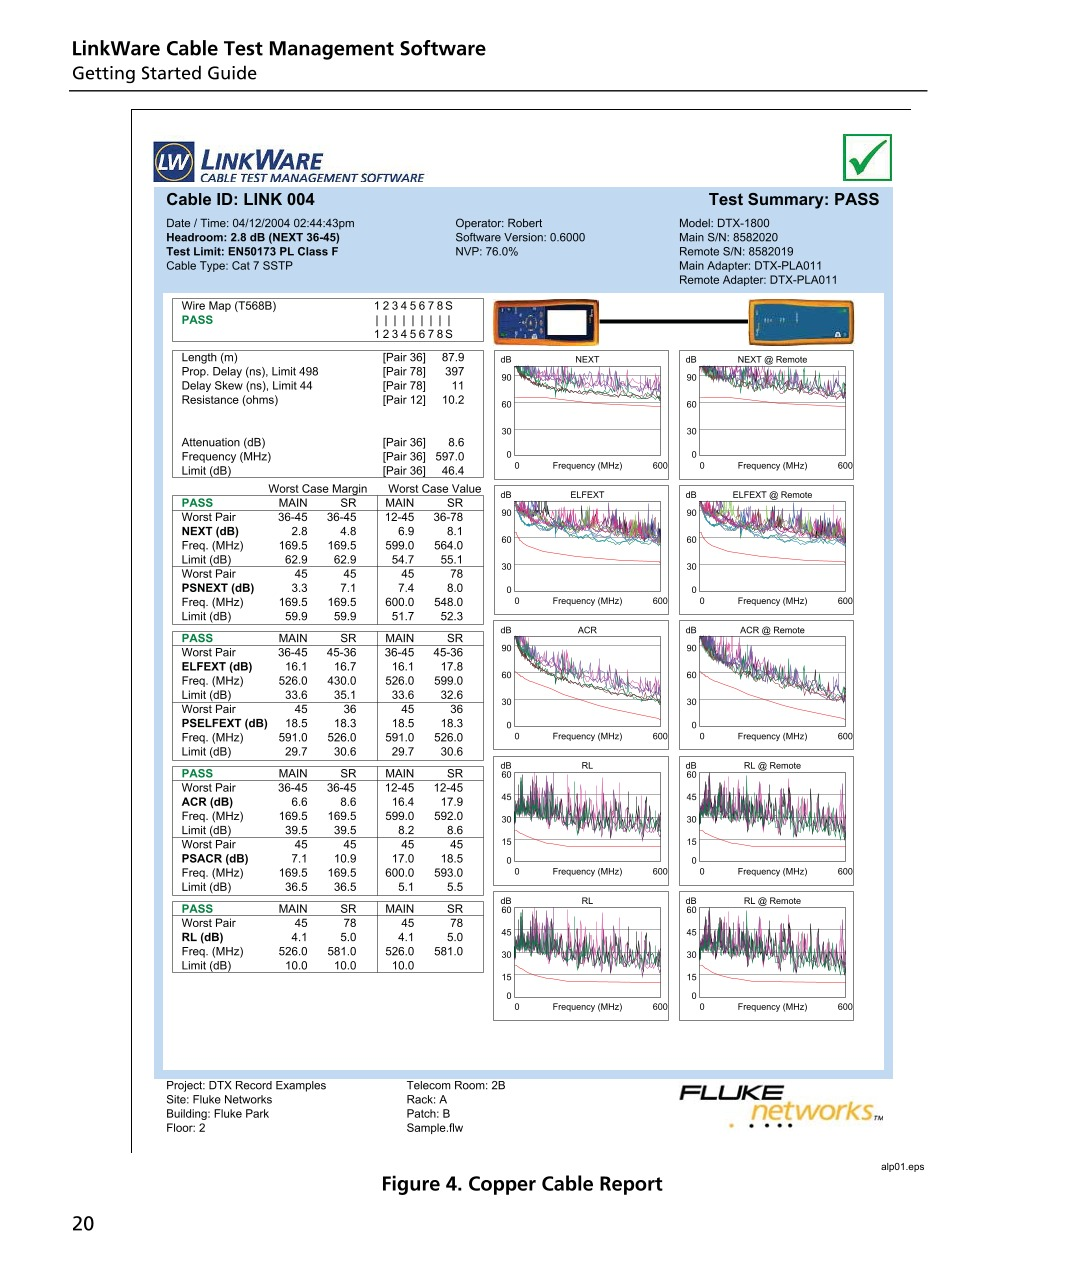
\includegraphics[width=\linewidth]{../images/0001.jpg}
  \label{fig:fluke-0001}
\end{figure}

\begin{figure}[H]
  \caption{Fluke Networks DTX-1800 reporte de cable de fibra óptica 1.}
  \centering
  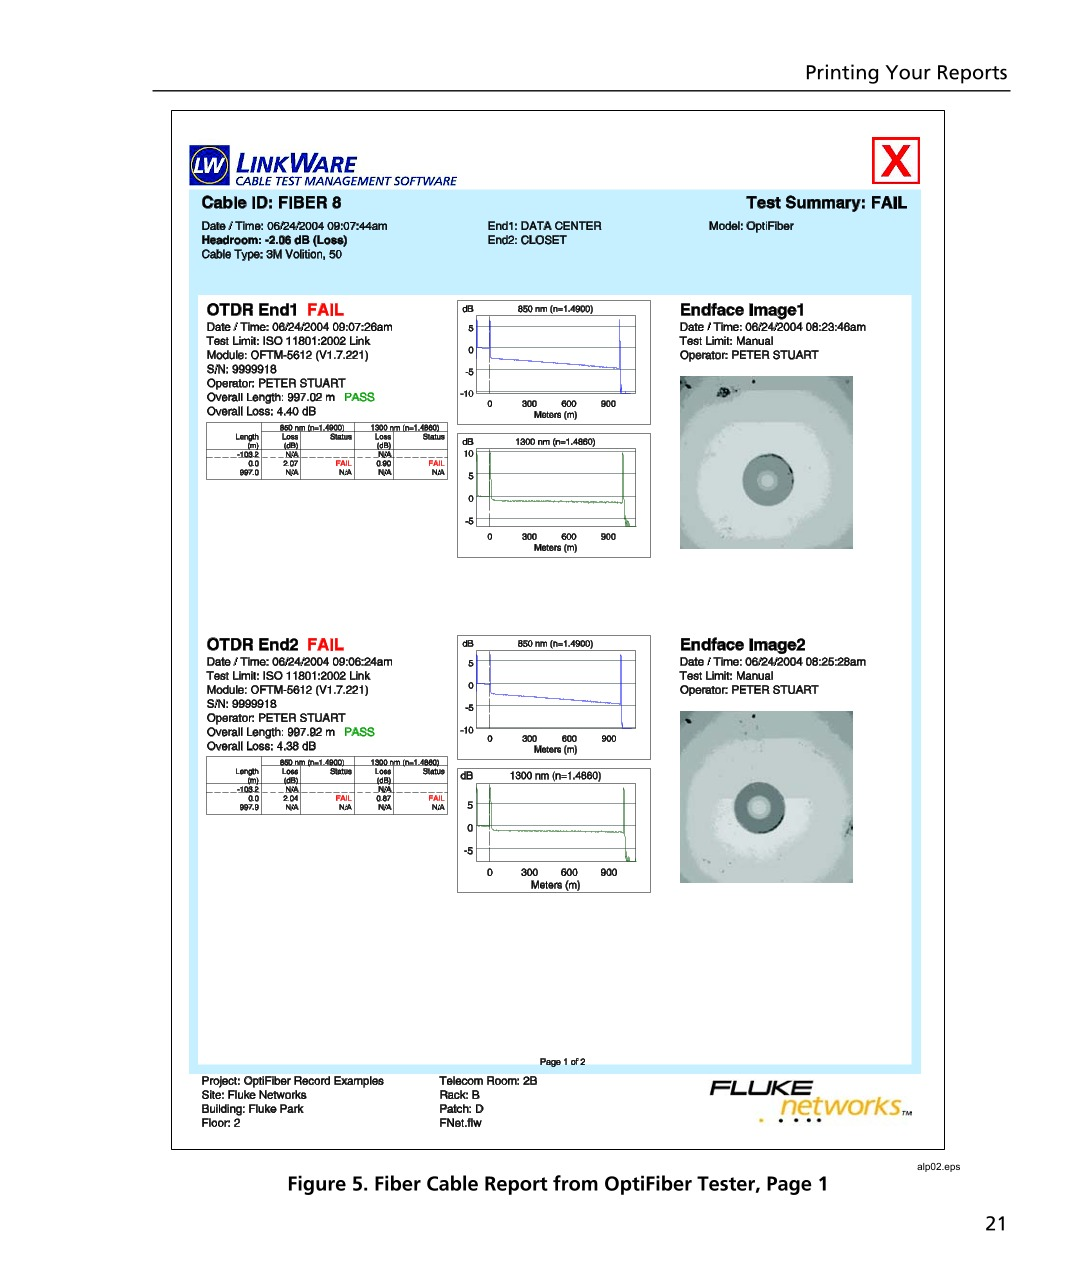
\includegraphics[width=\linewidth]{../images/0002.jpg}
  \label{fig:fluke-0002}
\end{figure}

\begin{figure}[H]
  \caption{Fluke Networks DTX-1800 reporte de cable de fibra óptica 2.}
  \centering
  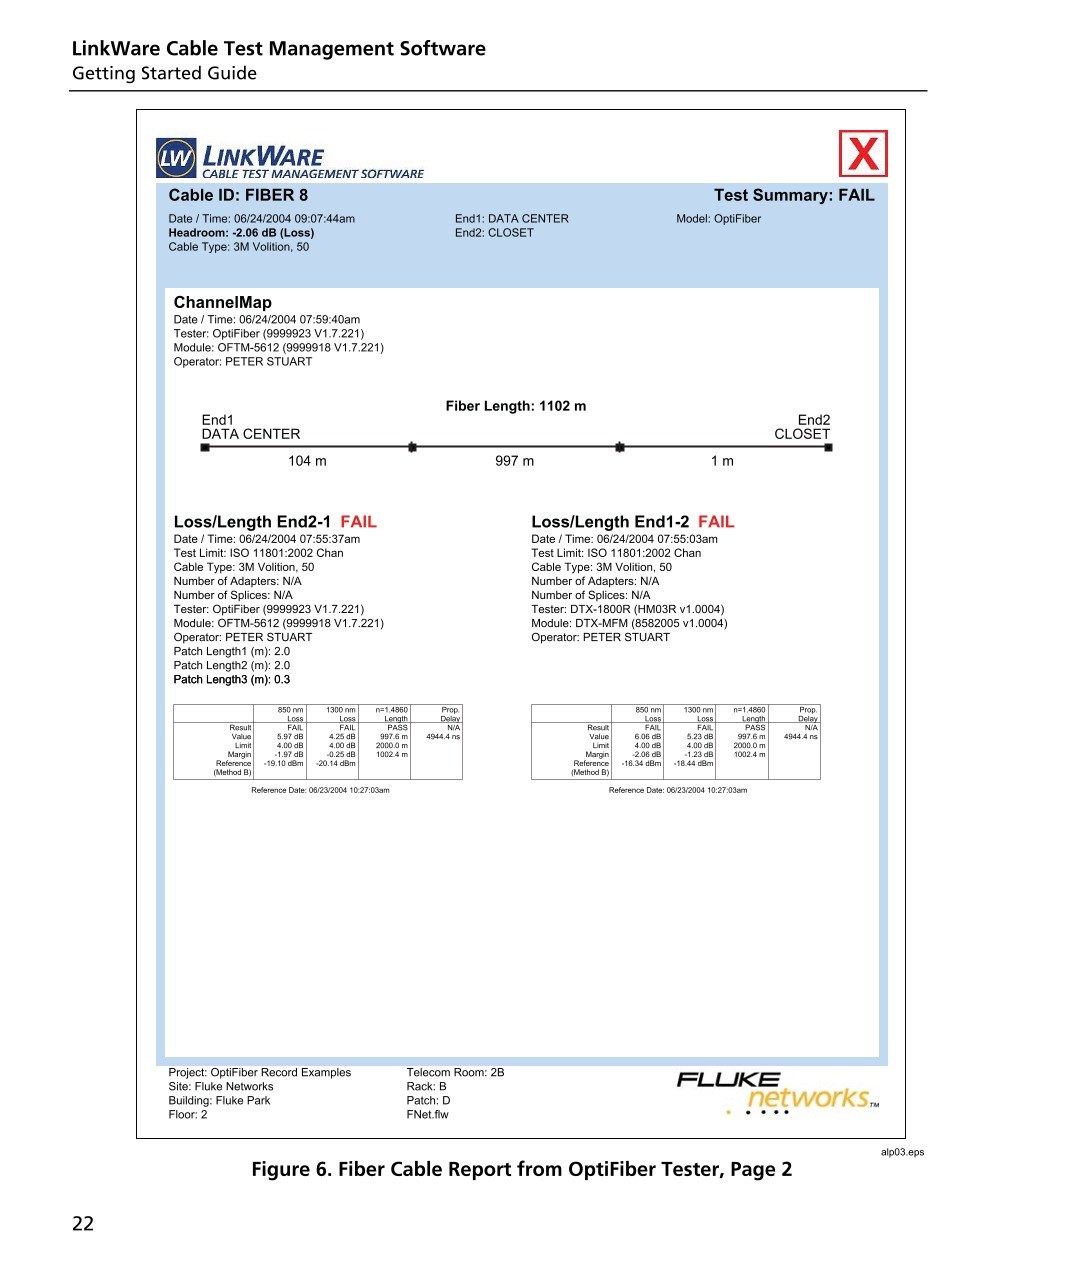
\includegraphics[width=\linewidth]{../images/0003.jpg}
  \label{fig:fluke-0003}
\end{figure}





